\chapter{Uživatelská rozhraní}
Grafická uživatelská rozhraní (GUI) jsou klíčovým prvkem většiny aplikací. Jsou to první, co uživatel uvidí a~co mu umožní s~aplikací interagovat. Dobře navržené GUI může znamenat rozdíl mezi úspěchem a~neúspěchem aplikace, proto by mělo být intuitivní, snadno ovladatelné a~příjemné na pohled. Následující kapitola bude věnována základním principům designu GUI.

\section{Stručná historie GUI}
Počátek grafických rozhraní se datuje do osmdesátých let minulého století, kdy firma \textit{Xerox} vyvinula počítač \textit{Alto}. Jednalo se o~první zařízení, jehož rozhraní se skládalo z~oken, ikon a~používalo myš k~ovládání. Toto grafické rozhraní pak posloužilo jako odrazový můstek a~základ dalším projektům. Jeden z~nich byl například \textit{Apple Macintosh}, který grafické uživatelské rozhraní popularizoval. Dále přišel operační systém \textit{Windows}, který GUI posunul ještě dál mezi mainstreamové uživatele. Toto odvětví se postupem let vyvíjelo společně s~novými technologiemi a~nyní je neoddělitelnou součástí téměř všech počítačových systémů.

\section{Zásady vývoje webového GUI}
Pro uživatelsky přívětivé UI je zásadní vzhled stránky a~použitelnost. Základní principy vychází z~praktických zkušeností grafiků i~psychologických studií.

\subsection{Vzhled stránky}
Tato sekce se bude věnovat základním principům designu, které by mělo moderní uživatelské rozhraní splňovat. Následuje několik z~nich, které jsou důležité pro vytvoření uživatelsky přívětivého GUI. \cite{principles_of_design}

\subsubsection*{Kontrast}
Kontrast, jakožto jedna z klíčových složek designu, zajišťuje, že text a~ostatní prvky jsou dobře čitelné a~viditelné. Jeho úlohou je posílit dojem a~upoutat pozornost na důležité prvky.

\subsubsection*{Vyváženost}
Každý prvek na stránce má určitou váhu, která je dána jeho velikostí, barvou, kontrastem a~dalšími faktory. Vyváženost zajistí, že tyto prvky jsou rovnoměrně rozloženy, což přispívá k~celkovému dojmu rovnováhy a~přehlednosti stránky.

\subsubsection*{Důraz}
Slouží ke zvýraznění důležitých prvků a~k~pomyslnému ukrytí těch méně podstatných. Můžeme tak kontolovat výraznost určitých informací a~zároveň usměrňovat pozornost uživatele.

\subsubsection*{Proporce}
Správně určené proporce podporují vyváženost a~harmonii na stránce. Uživatelům pomáhají orientovat se a~zajišťují, že stránka působí přehledně a~esteticky.

\subsubsection*{Hierarchie}
Hierarchie je podstatná, zejména pokud jde o~zdůraznění důležitých prvků. Tento princip je často demonstrován prostřednictvím titulů a~nadpisů. Titul stránky by měl okamžitě vyniknout jako nejdůležitější prvek, zatímco nadpisy by měly být formátovány tak, aby naznačovaly svůj význam ve vztahu k~sobě navzájem a~k~obsahu, který uvádějí.

\subsubsection*{Opakování}
Opakování je účinným nástrojem pro sjednocení myšlenek v~rámci designu. Lze ho dosáhnout konzistentním použitím barev, písma, tvarů nebo jiných prvků designu. Konzistentní formátování pomáhá sjednotit vzhled celé stránky.

\subsubsection*{Rytmus}
Slovem rytmus je myšlen styl, jakým jsou prvky (nebo jejich barvy, velikosti či dokonce mezery mezi nimi) na stránce uspořádány a~v~jakém pořadí použity. Některé rytmické vzory mohou vzbuzovat pocit uspořádanosti a~přehlednosti, zatímco jiné mohou působit chaoticky.

\subsubsection*{Vzory}
Vzory vyvolávají v~uživateli pocit předvídatelnosti a~pohodlí. Může se jednat například o~rozložení, které se běžně používá na jiných stránkách, nebo o~způsob zadávání dat, který je uživatelům známý.

\subsubsection*{Volný prostor}
Volný prostor (white space) je prázdné místo mezi prvky na stránce, který pomáhá zvýraznit důležité prvky a~zároveň zajišťuje, že stránka nevypadá přeplněná.

\subsubsection*{Navigace pohledem}
Jde o~kombinaci všech předešlých principů a~jejich aplikaci tak, aby uživatel mohl snadno a~pohodlně stránku použít.

\subsubsection*{Rozmanitost}
Může se jednat o~různé barvy, tvary či velikosti prvků, které zajišťují, že stránka nebude monotónní a~bude působit zajímavě.

\subsubsection*{Spojitost}
Spojitost zajišťuje, že všechny prvky na stránce působí jako celek. Většinou se jedná o~opakování barev či používání minimálního množství fontů.

\subsubsection{Teorie barev}
Výběr barev je nedílnou součástí vývoje každého GUI. Teorie barev se zabývá vztahy mezi barvami a~jejich významem. Poznáním těchto nuancí může vývojář využít vzhled stránky k~ovlivnění uživatelova vnímání své aplikace, neboť různé barvy mohou budit různý psychologický a~emocionální význam. Teorie barev poskytuje základní pravidla a~směrnice pro efektivní použití barev v~designu, aby se dosáhlo esteticky příjemného výsledku a~vyvolalo se požadované emoční nebo vizuální působení. Kromě toho také udává, že existuje několik kategorií základních barev:
\begin{itemize}
    \item \textbf{Primární barvy}: Červená, modrá a~žlutá. Tyto barvy nelze vytvořit kombinací jiných barev.
    \item \textbf{Sekundární barvy}: Zelená, fialová a~oranžová. Tyto barvy vzniknou smícháním dvou primárních barev.
    \item \textbf{Terciární barvy}: Těchto šest barev vznikne smícháním primárních a~sekundárních barvev. Patří sem například růžová, tyrkysová či žlutozelená.
\end{itemize}

Těchto dvanáct samozřejmě není jedinými barvami, které lze zejména u~moderních počítačů použít. Díky tomu se začal v~grafice používat takzvaný barevný kruh (color wheel). \cite{color_theory_design}

\subsubsection*{Barevný kruh}
Je často využíván pro své intuitivní uspořádání barev. Obsahuje kompletní paletu barev, které lze vytvořit smícháním primárních, a~umožňuje i~upravovat jejich odstíny přidáním černé či bílé. Existuje několik způsobů, jak pomocí tohoto kruhu vybrat vhodné barevné kombinace (některé z~nich můžeme vidět na Obrázku \ref{fig:color_theory}). \cite{color_wheel,color_schemes}
\begin{itemize}
    \item \textbf{Komplementární}: Barvy, které jsou proti sobě na kruhu, čímž vytvářejí kontrastní efekt.
    \item \textbf{Monochromatické}: Různé odstíny jedné barvy, což vytváří harmonický dojem.
    \item \textbf{Analogické}: Barvy umístěné na kruhu vedle sebe. Jejich kombinace vytváří přirozený a~pohodlný dojem. Je však vhodné vybrat jednu jako hlavní a~ostatní používat jako doplňky.
    \item \textbf{Triadické}: Kombinace tří barev, které na kruhu tvoří rovnostranný trojúhelník. Podobně jako způsob komplementární, také vytváří kontrastní efekt.
    \item \textbf{Rozštěpená komplementární}: Variace komplementární kombinace, kde se namísto jedné z protějších barev používají barvy s~ní sousedící.
    \item \textbf{Tetradické}: Čtyři barvy, kde vždy dvě z~nich tvoří komplementární pár -- na barevném kruhu vytváří obdélník. Pokud jsou barvy správně kombinovány lze dosáhnout jak kontrastního, tak harmonického efektu.
\end{itemize}

\begin{figure}[H]
    \centering
    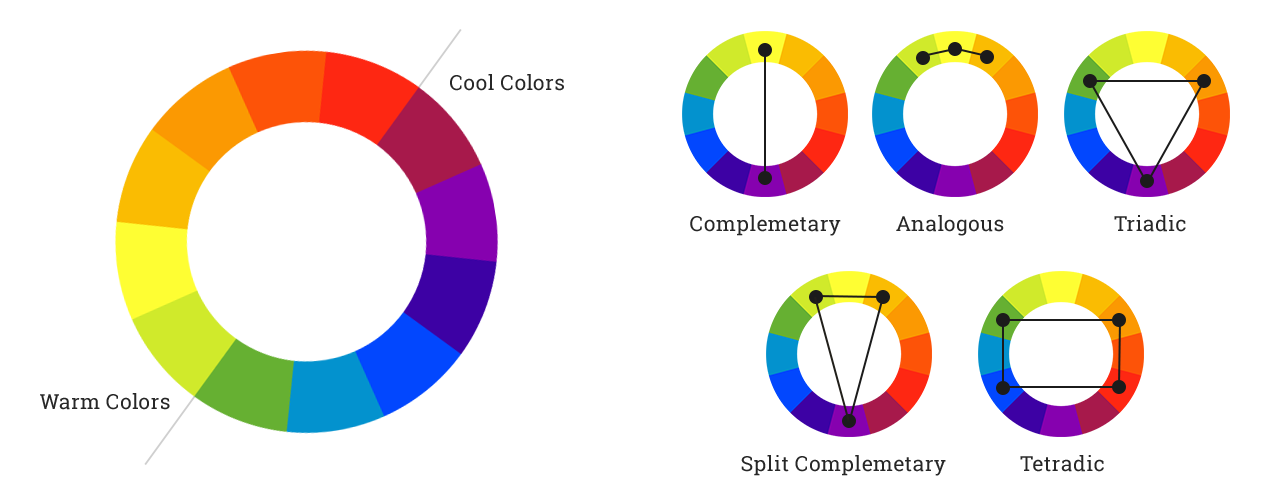
\includegraphics[width=0.9\textwidth]{resources/figures/color_theory.png}
    \caption{Barevný kruh a~dělení barev \cite{color_schemes}}
    \label{fig:color_theory}
\end{figure}

Dále se barvy dělí na teplé a~studené. Teplé barvy jsou červené, oranžové a~žluté části spektra a~často evokují radost a~energii. Studené barvy jsou zelené, modré a~fialové části, které často evokují klid a~harmonii. Výběr teplých či studených barev může mít vliv na celkový dojem, který uživatel z~aplikace získá. \cite{color_theory_design} 

\subsubsection{Typografie}
Typografie představuje umění používání písma a~fontů tak, aby text byl čitelný, srozumitelný a~příjemný k~čtení. Hraje klíčovou roli v~designu uživatelského rozhraní tím, že ovlivňuje rozpoznatelnost značky, uživatelovo rozhodování a~jeho pozornost. Kvalitní typografie přispívá k~efektivnímu předávání informací a~harmonické integraci s ostatními prvky rozhraní, což zlepšuje celkovou vizuální rovnováhu a~uživatelskou zkušenost. \cite{typography}

\subsection{Použitelnost}
Použitelnost je úzce spjata se vzhledem stránky a~často se tato témata překrývají, ale zároveň je to samostatný princip, který je nutné uvést zvlášť. Zahrnuje všechny aspekty, které usnadňují uživateli používání stránky. Níže jsou uvedeny ty nejdůležitější z nich. \cite{principles_of_ui_design}

\subsubsection*{Konzistence}
Pro uživatelskou přívětivost je konzistence téměř klíčová. Uživatel se rychleji naučí, jak stránka funguje, pokud je konzistentní. To znamená, že by vývojář měl dodržovat stejné rozložení a~navigaci mezi jednotlivými stránkami.

\subsubsection*{Zkratky}
Zkratky mohou urychlit a~tím zpříjemnit uživatelův pohyb po stránce. Tohoto výsledku můžeme dosáhnout například využitím odkazů v~menu či přesměrováním díky kliknutí na logo. Takovéto zkratky by měly být intuitivní a~měly by vycházet z~již známých vzorů.

\subsubsection*{Zpětná vazba}
Zpětná vazba je důležitá pro uživatele, aby věděl, zda se akce, kterou chtěl provést, zdařila či nikoliv, nebo jestli je možnost na nějaký prvek stránky kliknout. Tohoto dosáhneme pomocí animací, změny barvy či zvýraznění.

\subsubsection*{Uzavření dialogu}
Uzavření dialogu je podstatné, aby uživatel věděl, že jeho akce byla úspěšná a~může přejít k~dalším krokům. Tohoto můžeme dosáhnout například přesměrováním na jinou stránku či zobrazením dialogu, který uživateli potvrdí, že jeho akce byla úspěšná.

\pagebreak
\subsubsection*{Prevence chyb}
Zabezpečení proti nesprávným vstupům z~uživatelovy strany je podstatné pro předejití zbytečným chybám, které by mohly vést k~frustraci. K~tomuto přispějeme například tím, že nebudeme uživateli dovolovat zadávat písmena do pole, které by mělo obsahovat pouze čísla. Pokud už chyba nenávratně nastane, je důležité uživatele informovat o~tom, co se stalo a~jak jí může příště předejít.

\subsubsection*{Možnost vrácení}
Pokud se uživatel rozmyslí či udělá chybu, měl by mít možnost svou akci jednoduše zrušit a~vrátit se do předešlého stavu stránky.

\subsubsection*{Locus of control}
Tento fenomén by se dal volně přeložit jako těžiště řízení. Uživatelé chtějí mít pocit, že aplikaci řídí a~že rozhraní reaguje na jejich akce. Takového pocitu můžeme mimo jiné dosáhnout tím, že se zeptáme na potvrzení nějaké akce, například odchodu ze stránky s~neuloženými daty. Tím uživateli dáme pocit větší kontroly.

\subsubsection*{Minimalizace nároků na uživatele}
Klíčová zásada pro uživatelské rozhraní je minimalizace kognitivní zátěže. Ta může snížit uživatelovu schopnost vykonávat důležité úkoly, proto je podstatné, aby počítače převzaly co nejvíce úkonů na sebe. Uživateli můžeme vypomoci například zapamatováním si jeho přihlašovacích či osobních údajů, aby je nemusel zadávat při každém přihlášení. Při návrhu bychom měli vždy dávat přednost rozpoznání před vzpomínáním, abychom uživatelům umožnili rychle a~bez problémů dokončit své úkoly.

\subsubsection*{Responzivnost}
Jedna z~nejdůležitějších vlastností moderního GUI, responzivní design zajišťuje, že stránka bude vypadat dobře na všech zařízeních, od mobilních telefonů až po stolní počítače, a~to pomocí změny velikosti, schování či přesunutí prvků na stránce. K~tomu se využívají vlastnosti jazyka CSS, nejčastěji media queries, které umožňují nastavit jiné styly pro různé velikosti obrazovek. Responzivní design je v~dnešní době kriticky potřebný, protože většina uživatelů používá k~prohlížení internetu mobilní zařízení a~je důležité, aby se jim stránka zobrazila správně a~byla snadno použitelná. \cite{responsive_design}

\section{GUI ve vybraných hybridních hrách}
Tato sekce se bude věnovat analýze uživatelského rozhraní několika vybraných hybridních her. Jedná se o~hry, které jsou v~současné době populární a~mají velkou základnu hráčů. Analýza bude zahrnovat vzhled a~funkce GUI, které hry poskytují.

\subsection{Na vlnách neznáma}
Tato aplikace je vyvíjena a~udržována společností \textit{Plaid Hat Games}, která vydala i~samotnou hru. Jde o~oficiální rozšíření a~hlavní způsob, jak hru hrát. Společnost později vydala i~pdf dokument, které do určité míry tuto aplikaci nahrazuje, ale hráčům poskytuje méně možností. Jedná se o~webovou aplikaci, kterou je možné stáhnout a~používat offline, avšak bez některých funkcionalit, jako jsou například rozšíření či audio nahrávky.

\subsubsection*{Uživatelské rozhraní}
Kompaktní vzhled aplikace napovídá, že byla primárně určena pro mobilní zařízení -- je tedy i~bez velkých změn velmi dobře použitelná pro počítače. Jedná se o~jednostránkovou aplikaci s~jednoduchým a~přímočarým designem. Při spuštění uživatele přivítá logo hry a~přívětivě barevná grafika, která odpovídá fantasknímu námořnímu stylu hry. Samotná stránka obsahuje jen několik tlačítek; \textit{začít hrát}, \textit{nastavení}, \textit{ke stažení}, \textit{varianty hry} a~\textit{o~aplikaci}. Celá aplikace je přeložena do několika jazyků, a~to včetně češtiny.

\subsubsection*{Funkce}
Při spuštění hry se zobrazí výběr příběhové linky, kterou chtějí uživatelé zažít. Po vybrání se zobrazí stránka s~textovým polem, do něhož hráči mohou zadat číslo záznamu, který chtějí zobrazit. Toto číslo je jim oznámeno v~předešlém záznamu či v~knize lokací a~závisí na jejich dosavadních rozhodnutích. Aplikace také umožňuje zobrazit, jak mají hráči připravit herní plochu, statistiky jejich lodi a~karty. Na stránce je také možnost zapnutí odpočtu, pokud se hráči rozhodují moc dlouho, či náhled historie zobrazených záznamů.

Aplikace slouží převážně k~zobrazování výše zmíněných záznamů a~k~podporování imerze přehráváním ambientních zvuků a~audionahrávek s~narací příběhu. Mimo jiné také napomáhá s~událostmi ve hře, jako například v~boji tím, že za pomoci uživatelových vstupů kontroluje statistiky nepřátel.
 
\pagebreak
\subsection{Gloomhaven Secretariat}
Aplikace \textit{Gloomhaven Secretariat} je fanouškovským výtvorem, který vychází z~nyní již zrušené aplikace \textit{Gloomhaven Helper}. Jedná se o~jednostránkovou webovou aplikaci sestavenou v~\textit{Angularu}. Jde o~open-source software, na kterém se podílí množství fanoušků hry \textit{Gloomhaven} a~je stále ve vývoji. \cite{gloomhaven_secretariat_github}

\subsubsection*{Uživatelské rozhraní}
Aplikace je určena pro desktop či jiná zařízení s~velkou obrazovkou. Je sice použitelná i~na mobilních zařízeních, ale jedná se pouze o~zmenšenou verzi klasické stránky bez dalších úprav, což znamená, že některá tlačítka jsou příliš malá pro pohodlné používání. Obsah se také zdá být poměrné jednoduchý, avšak už není tak intuitivní, jako u~předešlého příkladu. Vzhled UI je čistě vypadající, a~navíc tematicky věrný samotné hře. Navigace po základní stránce je poměrně přímočará, avšak to stejné už se nedá říct o~rozsáhlých menu, které se skrývají téměř pod každým tlačítkem. Ty se mohou zdát na první pohled nepřehledné a~u~velké části z~nich je nedostatek popisků či vysvětlení, jak vlastně jednotlivá tlačítka fungují. Uživatel si tak musí nejprve odzkoušet, co vše je možné, což může být zdlouhavé a~frustrující. Zároveň bych však chtěl podotknout, že aplikace má tlačítko zpět, kterým může uživatel vrátit opravdu jakoukoliv akci, takže pokud hráč udělá nějakou chybu, je snadné ji napravit. Obdobně je zde i~tlačítko vpřed. Stránka také potřebuje neustálé vstupy od uživatele, aby dokázala správně plnit svou funkci, ty jsou však také někdy neintuitivní a~jejich zadávání často zdlouhavé a~repetitivní.

\subsubsection*{Funkce}
Hned na úvodní stránce dostane uživatel možnost výběru příběhové linie, kterou chce začít, a~následně ho stránka vyzve k~přidání postav. Dále je možnost přidat nepřátele postupně či spustit takzvaný scénář, což je v~pravidlech popsaná kombinace nepřátel, kteří se vyskytují v~určité části příběhu. Při boji aplikace zobrazuje statistiky postav a~nepřátel, jejich aktuální stavy a~efekty a~umožňuje je hráči kontrolovat a~upravovat. Stránka také sama náhodně vybírá z~možností nepřátelských akcí a~umožňuje hráčům za monstra \textquote{táhnout karty} a~tím udávat sílu a~efekt těchto akcí. Další možnosti aplikace zahrnují vedení globálních statistik skupiny, její úspěšnosti, odemčených lokací a~dalších věcí. Zároveň umožňuje ukládání a~stahování dat několika započatých her najednou.

Nutno říci, že aplikace je skutečně multifunkční a~nabízí hráčům velké množství automatizace a~ukládání dat. Tím velmi ulehčuje hru, zkracuje čas její přípravy a~zároveň zabraňuje chybám, které by mohly vzniknout při ručním vedení statistik.